%Z důvodu stochastičnosti modelu však může být nevýhodou velký rozptyl

%\chapter{Simulace epidemiologických opatření v modelu M}
\chapter[Simulace v multiagentním modelu]{Simulace epidemiologických opatření v multiagentním modelu}
\label{Evaluace_politik}

\textit{Petra Vidnerová, Gabriela Suchopárová, Roman Neruda}
\vspace{15mm}

Cílem této kapitoly je seznámit čtenáře s modelováním
epidemiologických opatření v multiagentním modelu M. Vysvětlíme
základní principy simulace jednotlivých opatření a ukážeme výsledky
dvou experimentů srovnávajících různé mechanismy trasování.


\section*{Úvod}

Během první vlny pandemie covid-19 šly mnohé státy včetně Česka
cestou tzv. lockdownu, kdy byly kontakty lidí omezeny až na
nejnutnější. Tento přístup byl účinný, avšak za cenu velkých
ekonomických ztrát. Pro další postup bylo tedy nutné zvolit šetrnější
opatření, která by nebyla tak ekonomicky nákladná, přesto by zabránila
šíření nákazy.

V praxi se však ukázalo, že zvolit vhodná opatření není
jednoduché. Při jejich zavedení dochází k omezení obyvatel a různých
odvětví, a je tedy nutné prokázat jejich účinnost a nutnost. Bez
zdůvodnění a analýzy jsou opatření zaváděna příliš pozdě, kdy už není
možné zabránit vyšším ztrátám na životech i poklesu ekonomiky.

Jedním z nástrojů, které mohou být nápomocny, jsou epidemiologické
modely. Ty je nutno rozšířit tak, aby umožňovaly modelovat skutečně
využívaná epidemiologická opatření, studovat jejich účinnost a
porovnávat zvažované varianty.

Epidemiologická opatření obecně snižují pravděpodobnost přenosu nemoci. Toho
je dosaženo buď omezením pravděpodobnosti, že při kontaktu s infekčním jedincem
dojde k přenosu nemoci (pomocí protektivních opatření jako rozestupy, roušky
a zvýšená hygiena), nebo omezením pravděpodobnosti, že k rizikovému kontaktu
dojde. Druhá skupina opatření omezuje samotné kontakty, a to buď plošně
(uzavření škol, obchodů, veřejných míst), nebo na individuální úrovni
(karanténa, izolace).




K efektivnímu omezení kontaktů na individuální úrovni je potřeba
aktivně dohledávat jedince, kteří přišli do kontaktu s nákazou. Proces
vyhledávání kontaktů nakažených je znám jako trasování a hraje
významnou roli v tlumení šíření nemoci. Řada epidemiologických modelů
obsahuje mechanismy pro modelování
trasování~\cite{pg:mooney2020,pg:kucharski2020,pg:Kerr2020,pg:keeling2020,pg:bilinski2020}.


Modelování různých epidemiologických opatření je i součástí 
modelu M~\cite{pg:modelM}. Základním nástrojem pro modelování trasování je v našem případě simulace.

V následující podkapitole stručně nastíníme základní principy modelu M
a vysvětlíme, jak jsou jednotlivá opatření v tomto modelu
simulována. Následuje podkapitola s ukázkou dvou experimentů
porovnávajících různě silné mechanismy trasování. V závěru shrneme
výhody a nevýhody našeho přístupu.


\section*{Metody}

\emph{Architektura epidemiologického modelu M.} Schéma modelu M je zobrazeno na obrázku~\ref{pg:fig:mm}. Model sestává ze
tří základních modulů -- epidemiologického modelu typu
SEIR~\cite{pg:bailey1975}, grafu kontaktů $G$ a {\em policy} modulu.

\begin{figure}[h]
  \centering
  \includegraphics[width=0.7\textwidth]{pic/model-m.eps}
  \caption{Schéma modelu M.}
  \label{pg:fig:mm}
\end{figure}



Jádrem modelu M je epidemiologický model typu SEIR. Pracuje s populací N
jedinců, kde každý jedinec je v jednom z možných stavů: $S$ -- zdravý jedinec,
který se může nakazit, $E$ -- nakažený jedinec, který ještě není infekční, $I$ --
infekční jedinec ($I_a$ presymptomatická fáze, $I_s$ symptomatická fáze, $I_n$
infekční bez symptomů),  $J$ -- nemocný jedinec, který už není infekční ($J_n$
asymptomatický, $J_s$ symptomatický), $R$ -- jedinec po prodělání nemoci, $D$ --
mrtvý jedinec.

Jedna iterace epidemiologického modelu odpovídá jednomu dni. Každý den
může dojít ke změně stavu jedince. Délky pobytů ve většině stavů jsou
dány parametry nemoci. Výjimku tvoří přechod $S \rightarrow E$, kde
je pravděpodobnost přechodu dána jak parametrem nemoci $\beta$
(nakažlivost), tak parametry hran příslušných uzlu odpovídajícímu
danému jedinci v grafu $G$.

Graf $G$ je další klíčovou komponentou modelu. V našem případě je
zkonstruován na základě reálných dat kontaktů mezi lidmi (odpovídá
skutečnému moravskému městu včetně přilehlých obcí, celkem cca 56 000
obyvatel). Jde o multigraf, kde mezi každými dvěma uzly (lidmi v daném
městě) může vést jedna nebo více neorientovaných hran. Ty představují
různé druhy kontaktů mezi dvěma lidmi. Hrana $e$ je dána trojicí $(l,
p, i)$, kde $l$ udává vrstvu (typ) hrany, $p$ je pravděpodobnost
kontaktu na dané hraně a $i$ je intenzita kontaktu. Celkem graf
obsahuje 30 vrstev (např. rodina, škola atd.), každá vrstva má svoji
váhu $w_l$. Váhy slouží jako pomůcka při simulaci plošných opatření,
jak ukážeme dále.

Pravděpodobnost, že na dané hraně dojde k nakažení (a jedinec tedy přejde z $S$
do $E$), je dána

\begin{equation}
  p_{S \rightarrow E}(e) = \begin{cases}
    \beta * i  & \mbox{pokud hrana je aktivní} \\
    0          & \mbox{pokud hrana není aktivní.} 
    \end{cases}
\end{equation}
Hrana je v dané iteraci aktivována s pravděpodobností kontaktu:
\begin{equation}
\label{pg:eq:w}
p_a(e) = w_l * p.
\end{equation}

Poslední částí modelu je {\em policy} modul. Volá se mezi každými dvěma
iteracemi jádra modelu a má možnost upravovat jak parametry samotného
epidemiologického modelu, tak modifikovat graf kontaktů $G$. Pomocí {\em policy} modulu
jsou implementovány různé politiky a opatření, např. testování a
trasování nebo karanténa. 

Více podrobností o samotném modelu M a sestrojení grafu kontaktů lze nalézt v~\cite{pg:modelM}.

\emph{Simulace epidemiologických opatření.} Popsaný model M umožňuje prostřednictvím {\em policy} modulu simulaci různorodých epidemiologických opatření.

Protektivní opatření (rozestupy, roušky apod.) realizujeme v modelu
redukcí parametru $\beta$, který reprezentuje nakažlivost nemoci.

Omezení kontaktů se pak implementuje pomocí redukce hodnot
pravděpodobností na příslušných hranách. V případě plošných opatření
jde pouze o změnu jednoho parametru, váhy příslušné vrstvy,
viz~(\ref{pg:eq:w}). Váhy vrstev jsou ve výchozím stavu rovny jedné a
umožňují jednoduše redukovat pravděpodobnosti všech hran spadajících
do dané vrstvy --  např. nastavením váhy na nulovou hodnotu vypneme
všechny kontakty v rámci dané vrstvy.

Při individuálním omezení kontaktů -- izolaci jednotlivých jedinců -- upravujeme jen
pravděpodobnosti hran patřících danému uzlu, který je izolován. To znamená, že
vezmeme každou hranu $v$ tohoto uzlu a upravíme její pravděpodobnost:
$$
p_{v_{new}} \leftarrow p_{v} * q_l,
$$
kde  $l$  je vrstva hrany  $v$. 
Koeficienty izolace $q_l$ lze nastavit např.
$$
q_l =
\begin{cases}
  1  &  \mbox{pokud } l \mbox{ je vrstva na úrovni rodiny} \\
  0  &  \mbox{jinak,}
\end{cases}
$$
kde hrany odpovídající rodině zůstávají beze změny a ostatní hrany jsou vypnuty. Použitím nenulových hodnot $q_l$ pro vybrané vrstvy lze simulovat částečné dodržování karantény, a to pouze na určitých vrstvách (např. $0.5$ pro rodinné návštěvy, ale $0$ pro návštěvy restaurací apod.). 


Samotný proces testování a trasování je v modelu implementován pomocí {\em policy} modulů. Jednou z implementovaných politik je tzv. samoizolace. Uzel,
u kterého se projeví příznaky, je s určitou pravděpodobností izolován. Tato
izolace odpovídá v realitě skutečnosti, že pacient s příznaky se sám rozhodne
zůstat doma (aniž byl pozitivně otestován).

Další implementovaná politika realizuje testování. Uzel, u kterého se
projeví příznaky, se s určitou pravděpodobností ($test\_rate$)
rozhodne jít na test. Pokud se rozhodne kladně, každý další den se
určuje pomocí parametru $\theta_{I_s}$, zda se na test
dostal. Nastavení $\theta_{I_s}$ je provedeno na základě skutečné
prodlevy mezi prvním příznakem a testem z historických dat. V případě
pozitivního výsledku testu je daný uzel izolován.

Poslední ze základních politik je trasování. Cyklus, kterým může testovaný a
vytrasovaný uzel projít, je znázorněn na obrázku~\ref{pg:fig:ct}. Uzel, který je
pozitivně otestován, je izolován, poté je dotázán na své kontakty. Model udržuje
databázi uskutečněných kontaktů (aktivních hran) pro posledních 14 iterací (dní). V této databázi jsou vyhledány hrany, jejichž součástí je pozitivně
otestovaný uzel a které nejsou starší než dva dny před projevením příznaků.

V reálném světě nikdy nedojde k dohledání všech kontaktů, neboť na některé si dotyčný vzpomene, avšak na jiné zapomene. Proto jsou tyto vyhledané hrany dále
profiltrovány. Každá vrstva má svoji pravděpodobnost \uv{vybavení si} hrany a s touto
pravděpodobností hrana zůstává v seznamu. Pro jednoduchost rozdělujeme vrstvy
do čtyř skupin -- rodina, škola a práce, volný čas, ostatní. Sílu trasování pak
udáváme čtveřicí pravděpodobností $(p_1, p_2, p_3, p_4)$, kde 
$p_1$ udává pravděpodobnost vybavení si kontaktu na vrstvě rodina, $p_2$
pravěpodobnost vybavení si kontaktu, který proběhl na vrstvě spadající pod školy
nebo práci, atd.


Výsledný seznam pak umožňuje získat kontakty -- uzly, které jsou izolovány (je na
ně uvalena karanténa). To nastane s prodlevou dvou dnů, která simuluje časovou
náročnost trasování a telefonického zkontaktování vytrasovaných osob.
Příslušné uzly jsou testovány (pět dní po kontaktu nebo druhý den, pokud uběhlo
více dní) a pozitivně testované uzly jsou také podrobeny procesu trasování. 
Všechny uzly, které jsou v izolaci, jsou uloženy v databázi izolací spolu s délkou
své izolace. Tato délka je při každé iteraci {\em policy modulu} (každý den)
snížena o jedna. Po uplynutí požadované délky izolace je provedena výstupní
procedura, a pokud uzel splňuje její podmínky, je izolace ukončena (hrany uzlu
jsou navráceny do původního stavu, ale jen za podmínky, že uzly na druhém konci
nejsou izolovány). Příkladem podmínky ukončení izolace jsou dva negativní testy s
odstupem dvou dnů nebo uplynutí určité doby od pozitivního testu.


\begin{figure}
  \centering \includegraphics[width=0.9\textwidth]{pic/contact_tracing.eps}
  \caption{Schéma algoritmu testování a trasování kontaktů.}
  \label{pg:fig:ct}
\end{figure}




\section*{Výsledky}
Jako příklad použití popsaného modelu uvedeme dva experimenty porovnávající
různě silné mechanismy trasování. Pro každé nastavení bylo provedeno 1000
simulací pro pevně daná různá počáteční nastavení náhodného
generátoru (což zaručí různý průběh každé simulace, který je však díky nastavení možné kdykoli zopakovat).

V experimentech uvažujeme pět hypotetických trasovacích algoritmů o
síle $(0, 0, 0, 0)$ (žádné trasování), $(1, 0, 0, 0)$ (trasuje se
pouze rodina), $(1, 1, 0, 0)$ (trasují se rodina, školní a pracovní
kontakty), $(1, 1, 1, 0)$ (trasuje se vše kromě kategorie ostatní) a
$(1, 1, 1, 1)$ (ideální trasování). Ideální trasování odpovídá použití
elektronické trasovací aplikace, která umožňuje dohledání kontaktů
osob mimo okruh známých (rodiny, přátel, spolupracovníků atd.) trasovaného jedince. Pro zjednodušení
uvažujeme stoprocentní úspěšnost trasování dané skupiny kontaktů.

V prvním experimentu bylo použití těchto trasovacích algoritmů
simulováno jak v situaci bez jakýchkoli plošných uzávěr (viz
obr.~\ref{pg:fig:exp1a}), tak v situaci s plošnými uzávěrami
odpovídajícími situaci v České republice na jaře 2020 (viz
obr.~\ref{pg:fig:exp1b}). K nastavení vah jednotlivých vrstev pro
simulaci reálných plošných uzávěr byla použita data ze sociologického
výzkumu~\cite{pg:paqcovid}. Nošení roušek a další protektivní opatření
jsou fixována na hodnotu $0.5$ (na škále $0 - 1$, kde $0$ odpovídá
žádným protektivním opatřením a $1$ maximálnímu dodržování nošení
roušek a ostatních protektivních opatření).

Výsledky jsou zobrazeny na obrázcích~\ref{pg:fig:exp1a}
a~\ref{pg:fig:exp1b}, které zobrazují medián a mezikvartilové rozpětí
průběhů epidemie z 1000 provedených simulací.



\begin{figure}[ht!]
  \centering
  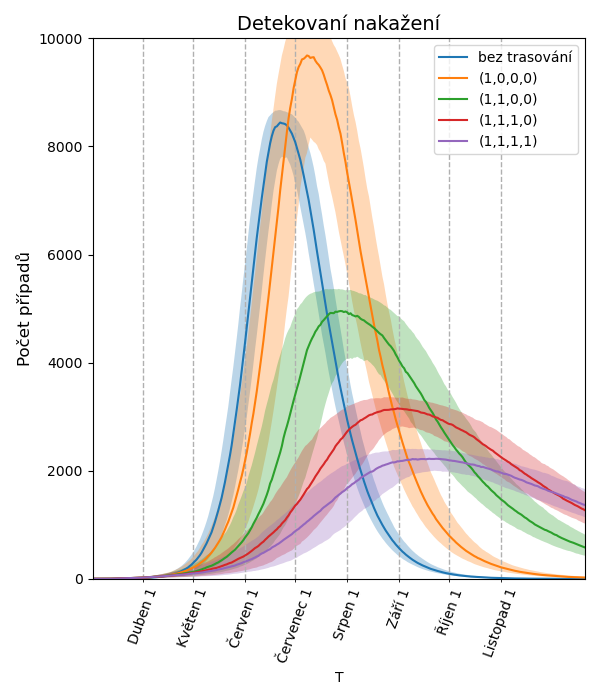
\includegraphics[width=0.45\textwidth]{pic/history_second_exp_detected_iqr.png}
  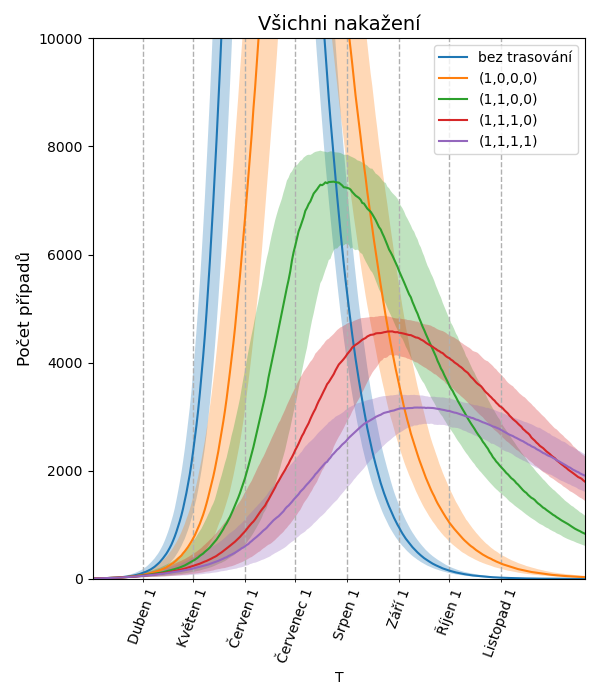
\includegraphics[width=0.45\textwidth]{pic/history_second_exp_all_iqr.png}
  \caption{Srovnání průběhů epidemie pro různé síly trasování.}
  \label{pg:fig:exp1a}
\end{figure}

\begin{figure}[h!]
  \centering
  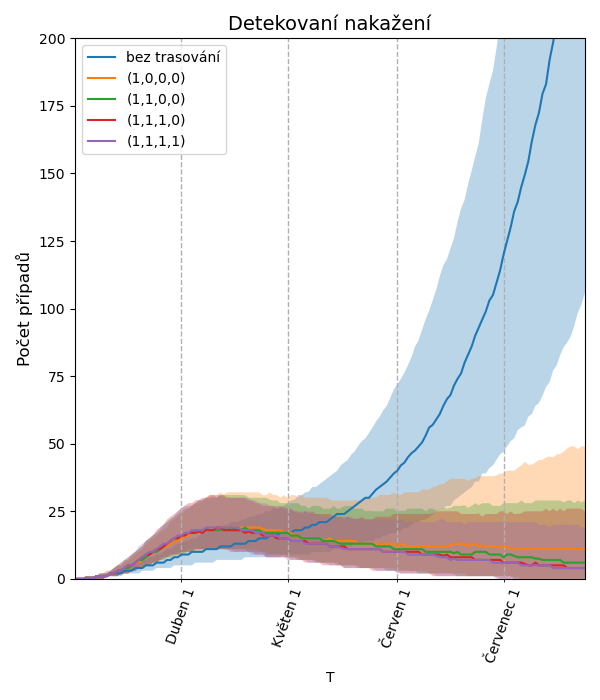
\includegraphics[width=0.45\textwidth]{pic/history_second_expB_detected_iqr.png}
  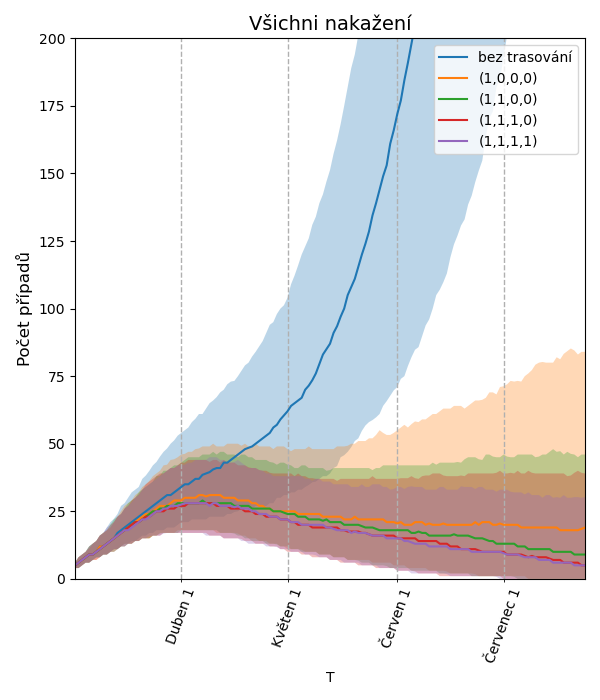
\includegraphics[width=0.45\textwidth]{pic/history_second_expB_all_iqr.png}
  \caption{Srovnání průběhů epidemie pro různé síly trasování na pozadí plošných opatření.}
  \label{pg:fig:exp1b}
\end{figure}

\begin{figure}
  \centering
  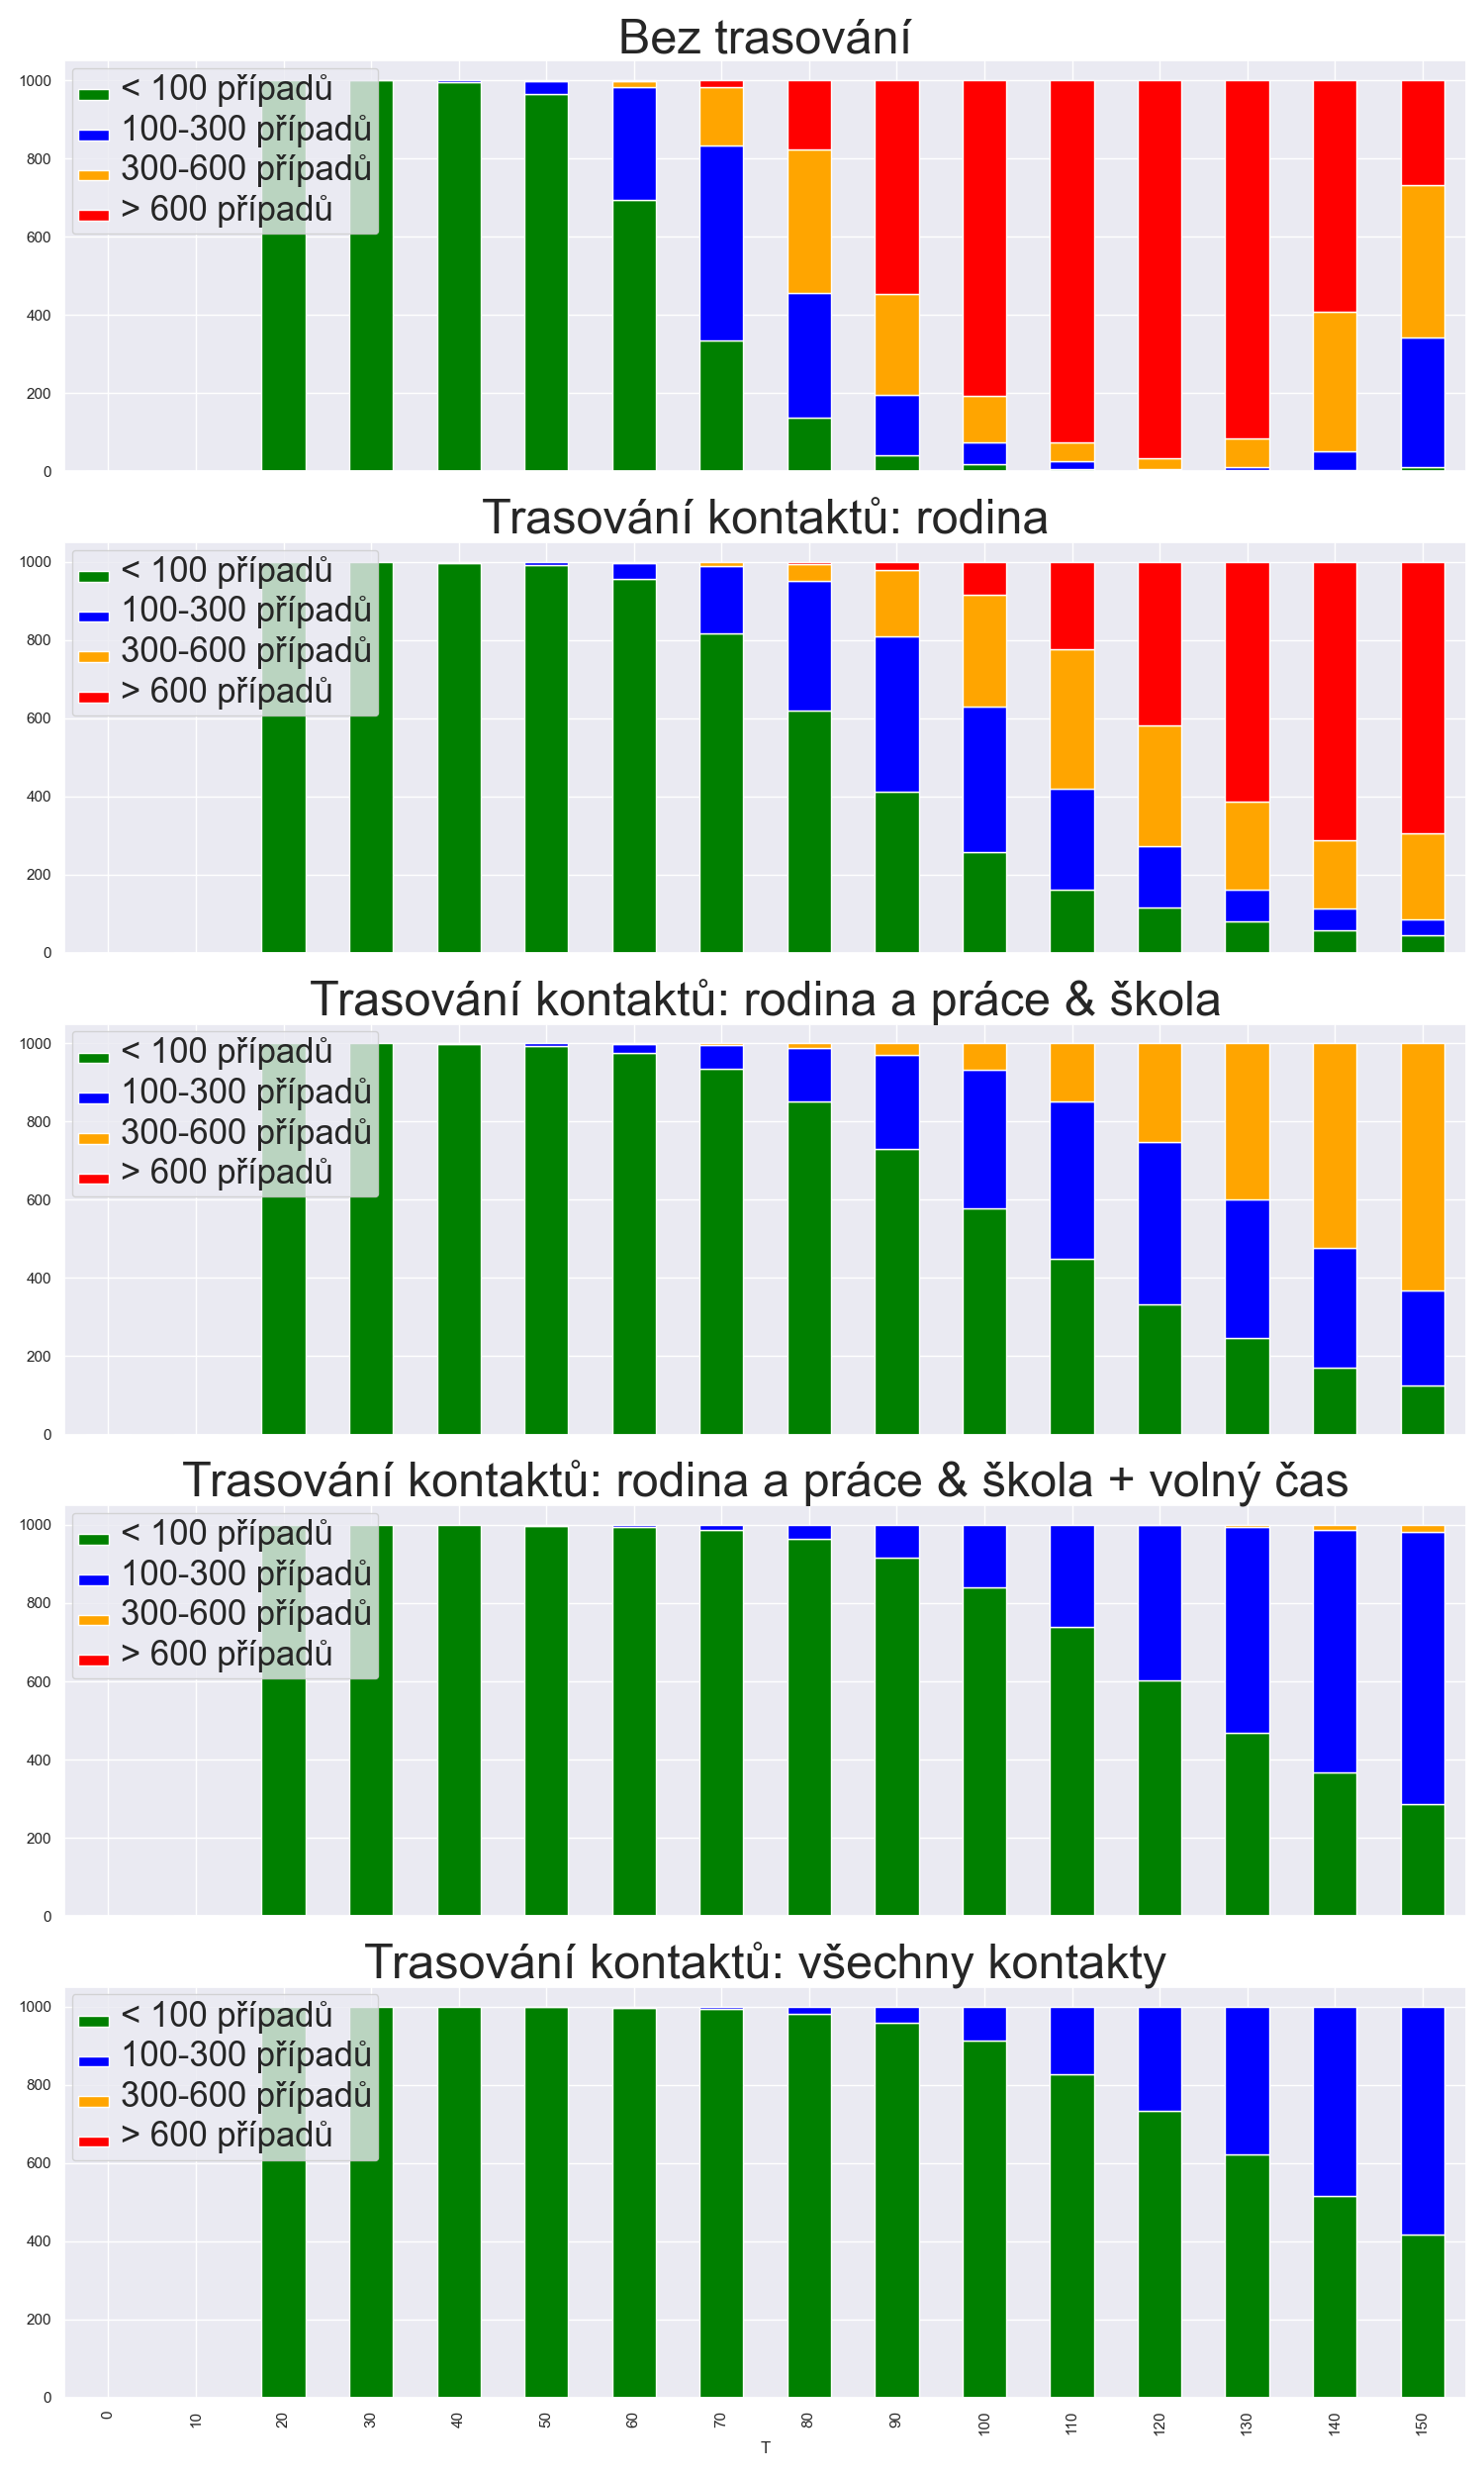
\includegraphics[width=0.49\textwidth]{pic/bar_prubeh_history_second_exp.png}
  \hfill
  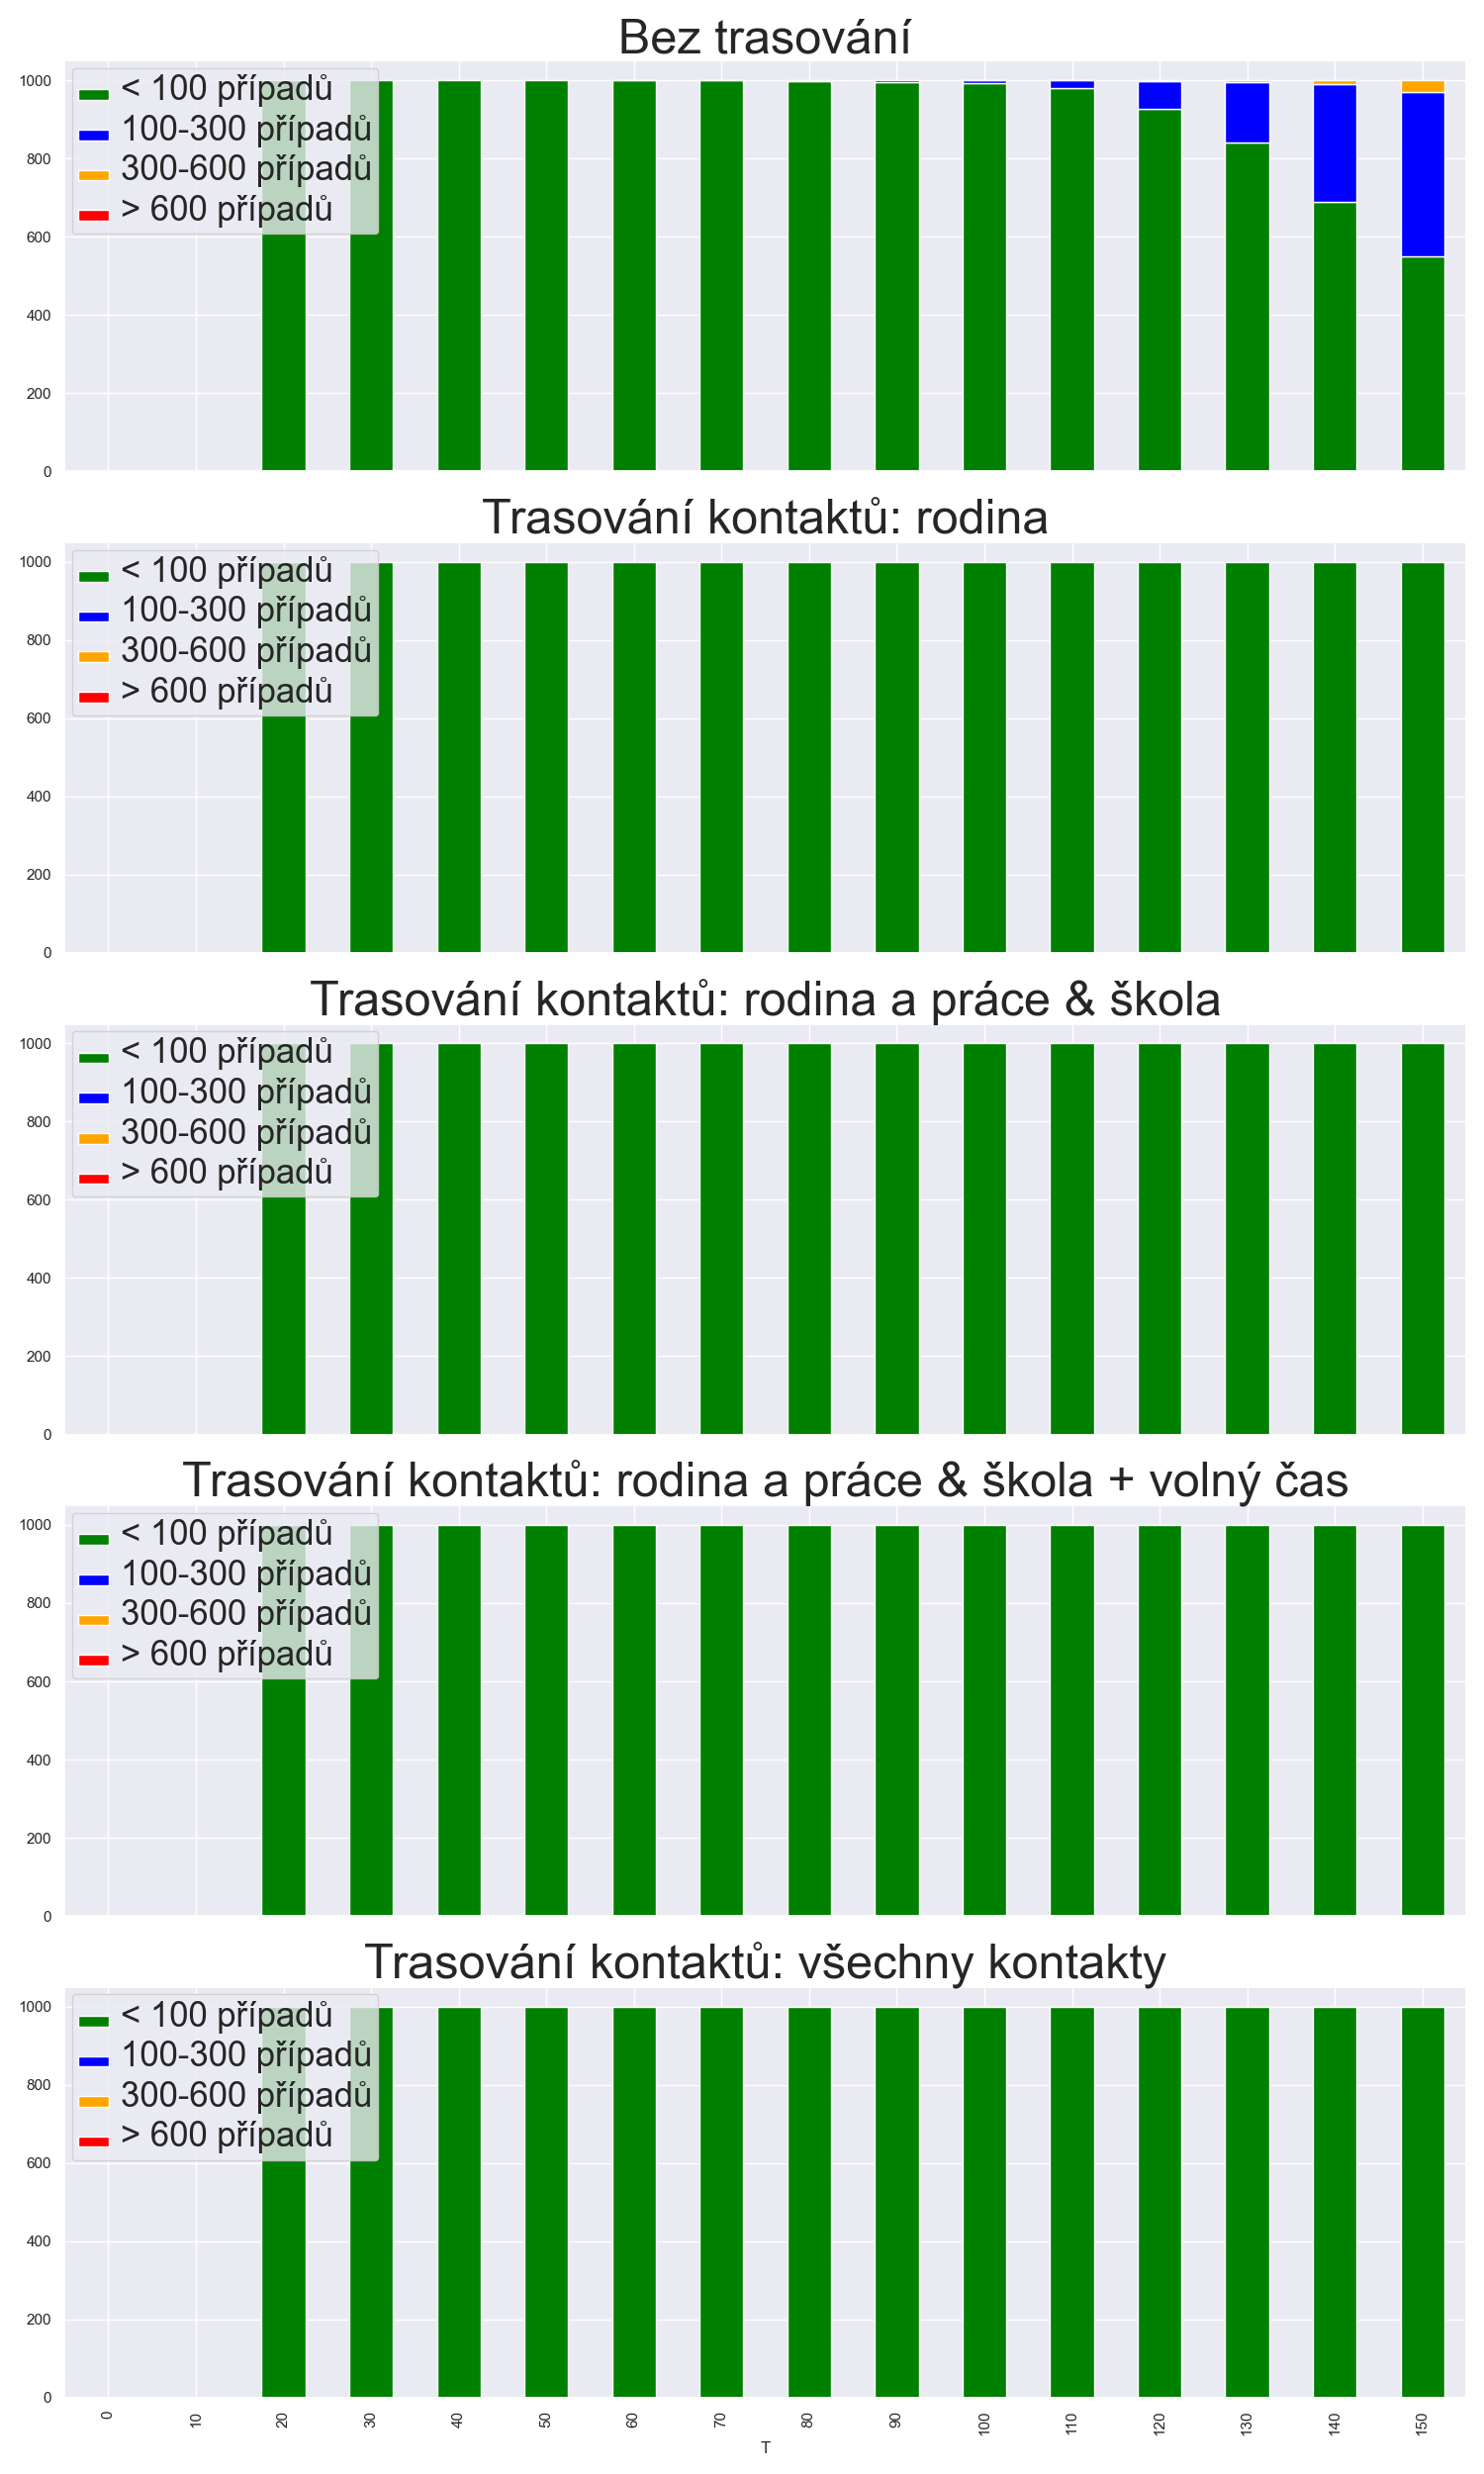
\includegraphics[width=0.49\textwidth]{pic/bar_prubeh_history_second_expB.png}
  \caption{Rozdělení 1000 běhů simulace epidemie dle závažnosti (barevného {\em
      semaforu}) v čase (osa $x$ -- den simulace). Zelená: méně než 100 nových
    případů, modrá: 100 až 300 nových případů, oranžová: 300 až 600 nových
    případů, červená: více než 600 nových případů. Počet nových případů je
    přepočtený na celou Českou republiku a jde o klouzavý průměr za 14
    dní. Nalevo: scénář bez plošných opatření, napravo: scénář s plošnými omezeními.}
  \label{pg:fig:exp1ab}
\end{figure}


Na obrázku~\ref{pg:fig:exp1a} vidíme důležitost jednotlivých trasování při
velké epidemii bez jakýchkoli plošných omezení. V takovém případě
nestačí trasování rodiny, ale je nutné k utlumení epidemie přidat i
pracovní, školní a volnočasové kontakty. Ideální trasování již
nepřináší tak výrazné zlepšení oproti tomuto typu trasování.

Obrázek~\ref{pg:fig:exp1b} přináší srovnání stejných trasovacích
mechanismů v situaci s plošnými omezeními (odpovídajícími jaru 2020 v
České republice). I v případě plošných omezení je trasování nutné,
neboť bez něj dochází ke vzestupu epidemie. V tomto případě
se však rozdíly mezi slabým a silným trasováním stírají a i trasování
pouze rodinných kontaktů je dostatečné k udržení nízkého stupně epidemie. 

Pro lepší představu o rozložení jednotlivých běhů simulace je na
obrázku~\ref{pg:fig:exp1ab} zobrazena klasifikace běhů dle závažnosti
epidemie. Zelená barva označuje běhy s mírnou epidemií, červená naopak běhy,
kde epidemie závažně roste. Klasifikace je založena na klouzavém průměru
nových případů. Osa $x$ odpovídá dni simulace, vertikálně je pak vyneseno
všech 1000 běhů. Vidíme opět, že plošná opatření jsou silná, a ke vzestupu
epidemie dochází pouze v případě bez jakéhokoli trasování. 


Druhý experiment porovnává uvedených pět trasovacích algoritmů ve
scénáři, kde je povoleno konání velkých akcí za přítomnosti mnoha
lidí. V našem případě je to akce pro 300 lidí, kteří se blíže
neznají. Tato akce se koná jednou týdně. Na obrázku~\ref{pg:fig:exp2}
vidíme porovnání histogramů počtu nakažených ve 100. dnu epidemie pro
jednotlivé trasovací algoritmy (každý histogram odpovídá 1000
simulací jedné trasovací strategie). Viditelný rozdíl je v tomto
případě i mezi silným trasováním $(1, 1, 1, 0)$ a ideálním trasováním
$(1, 1, 1, 1)$. Ideální trasování umožňuje dohledat i rizikové
kontakty uskutečněné na hromadné akci, které v tomto scénáři hrají
významnou roli v šíření nákazy.

\begin{figure}[ht!]
  \centering
  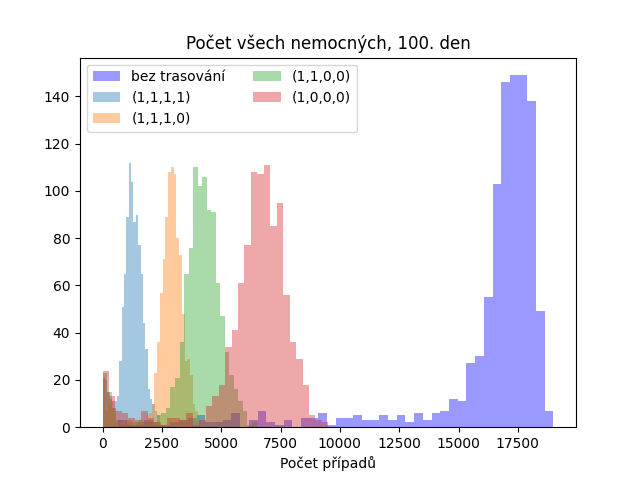
\includegraphics[width=0.6\textwidth]{pic/histogram_party2.png}
  \caption{Histogram  počtu nakažených ve 100. dnu epidemie pro jednotlivé trasovací algoritmy.
  Na vodorovné ose je počet nakažených ve 100. dnu běhu simulace, na svislé ose počet odpovídajících simulací.}
  \label{pg:fig:exp2}
\end{figure}


\section*{Závěr}

Uvedené experimenty ilustrují možnosti použití našeho modelu a
ukazují, že aktivní opatření mají velký vliv na průběh epidemie. Z
prvního experimentu je vidět velká síla plošných opatření i nutnost
důslednějšího trasování při jejich nepřítomnosti.

Druhý experiment ilustruje přínos elektronických trasovacích aplikací
typu {\em eRouška} při konání velkých akcí, kde se lidé vzájemně
neznají.

Oba experimenty ukazují i jednu nevýhodu našeho modelu, a to velký rozptyl 
výsledných průběhů simulované epidemie způsobený stochastičností modelu (viz mezikvartilové rozpětí na
obrázcích~\ref{pg:fig:exp1a} a~\ref{pg:fig:exp1b} nebo šíře histogramů
na obrázku~\ref{pg:fig:exp2}). Proto je vždy nutno provést větší množství
simulací, což s sebou nese větší výpočetní náročnost.

Další obtíží, která vychází z podstaty modelu, je velké množství parametrů. Část lze nastavit na základě
již známých znalostí chování nemoci covid-19, část (především parametr $\beta$) je nutno dohledat pomocí simulací historie průběhu epidemie (minulosti). Toto dohledání obnáší evaluaci velkého množství nastavení modelu a výběr těch nastavení, kde se průměrný simulovaný průběh shoduje se skutečností. Tato fáze je výpočetně velmi náročná a používáme k ní počítačový cluster s větším množstvím procesorů. 

Není však třeba reprodukovat minulý průběh s naprostou přesností, protože model sám není určen k samotné predikci průběhu epidemie, ale spíše má sloužit jako nástroj pro relativní srovnávání jednotlivých opatření. 

Jeho hlavní výhodou je možnost simulace jak plošných opatření, tak
opatření individuálních. Současně je možno simulovat dodržování
opatření protektivních (redukcí parametrů nakažlivosti). Díky
struktuře modelu mohou být opatření simulována detailně (na úrovni
kontaktu dvou lidí). Lze simulovat různě silné mechanismy testování
(na úrovni vrstev) a různé stupně izolace (různá síla oslabení hran
na jednotlivých vrstvách).


Modulární struktura modelu umožňuje implementovat další opatření a
politiky na míru požadovanému experimentu. Pomocí jiného {\em policy}
modulu lze modelovat očkování. Výměnou grafu lze simulovat odlišné
prostředí a aplikovat jemu specifické politiky (např. rotace a testování
ve školách).


Implementace modelu je dostupná na~GitHubu \cite{pg:mmsoft}.

